%Semiconductors_Transduction
\chapter{Semiconductors and Transduction}
We have studied devices that follow Ohm's law. But not all electrical
elements follow Ohm's law. And many Non-ohmic devices are very useful. Your
cell phone is full of non-ohmic devices and so is your computer. We will
study one of these today, a semiconductor PN junction or a diode. We have
already seen light emitting diodes (LEDs) used as light sources that we
could turn on and off. But today we will use this non-ohmic device to
convert light energy into a electrical signal!

To convert energy from one form to another is called \emph{transduction}.
There are thousands of different types of transducers. Even in your own body
you have sound, light, pressure, and chemical energy transducers that
convert sound, light, pressure, and chemical energy to nerve signals. In
lab, we will convert such energies to electrical signals that our meters or
Arduino DAQs can detect. We will choose just one today, the transduction of
light energy to electrical signals using a diode.

\section{The Model to Test}

The model that we will test comes from the end of PH220. And it is a simple
model. For a point light source, the intensity of light goes like 
\begin{equation*}
I=\frac{P}{4\pi r^{2}}
\end{equation*}%
where $P$ is the output power and $r$ is the distance from the point source
to the detector. Our model says that from a point source the light energy
will go out equally in all directions. \begin{figure}[h!]
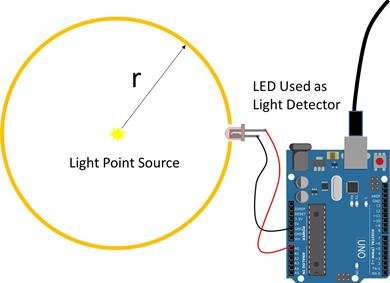
\includegraphics[width=3.2872in,height=2.3895in]{PH4CAX3S}
\end{figure}

We have some old-fashioned light bulbs that we can use as light sources.
They conveniently have the power that they use marked on them. So what we
expect from our model is that the intensity of the light from the bulb
should decrease with distance like $1/r^{2}.$

\section{The Instrument}

We will allow light from the bulb to strike our diode. If the light is the
right color (has the right energy per photon) it can knock an electron loose
in the inner workings of the diode (see the section \ref{Semiconductors} for
more details on how this works). When this happens, a small current is
formed (very small, one electron is moving). If we have more light, then we
can create a steady current. It will still be small, but will be measurable,
about $2.5\unit{nA}$. To measure our current, we will use our Arduino
directly, which may sound a bit strange. But our Arduino has an internal
resistance inside of it. That internal resistance is not small! It is on the
order of $10\unit{M%
%TCIMACRO{\U{3a9}}%
%BeginExpansion
\Omega%
%EndExpansion
}.$ With this large resistance, we expect a voltage of around 
\begin{eqnarray*}
\Delta V &=&IR \\
&=&2.5\unit{nA}\times 10\unit{M%
%TCIMACRO{\U{3a9}}%
%BeginExpansion
\Omega%
%EndExpansion
} \\
&&0.025\unit{V}
\end{eqnarray*}%
With our simple Arduino voltmeter we have an uncertainty of 
\begin{eqnarray*}
\delta V_{\min } &=&4.9\unit{mV} \\
&=&0.004\,9\unit{V}
\end{eqnarray*}%
so we expect to be able to see this voltage. And the voltage is proportional
to the current. And the current is proportional to the light intensity. This
means that we can make a light detector with just a diode and an Arduino!
That is just what we are going to do.

The circuit is super simple. Just wire the LED between the GND and AO pins.
It might be helpful to use a prototyping board so that you can handle the
instrument more easily. If you do use a proto-board, you will need some
wires. But still, the instrument is very simple.

There are some things we need to know, however. The LED is sensitive to
light of just one wavelength. Our light bulbs will give us many wavelengths.
So we won't detect all the light power. Also the LEDs we have are in little
plastic cases. The plastic cases are curved on top, which makes them a lens. 
\begin{figure}[h!]
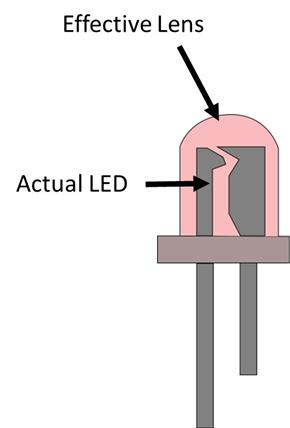
\includegraphics[width=1.5394in,height=2.2667in]{PH4CAX3T}
\end{figure}The lens makes the LED detector
very directional. You have to point the LED\ right at the light. I\ measured
the angular dependence of one of our LEDs by placing the LED at about $30%
\unit{cm}$ from the light bulb and then rotating it in $5\unit{%
%TCIMACRO{\U{b0}}%
%BeginExpansion
{{}^\circ}%
%EndExpansion
}$ increments. Here is what I found: \begin{figure}[h!]
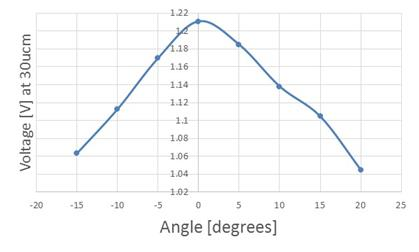
\includegraphics[width=3.5293in,height=2.13in]{PH4CAX3U}
\end{figure}If we are about $15$ degrees off,
we lose about $12\%$ of our voltage. Since the model we are testing tells us
voltage goes down with distance, we will have to be very careful to not
misinterpret a voltage drop as due to distance when really it is just that
we didn't aim well! It is probably worth using a ring stand or something and
taping your proto-board or Arduino to the stand to give stability to the
set-up.

Though we are measuring amount of light, our Arduino is just acting as a
simple voltmeter. The sketch is very simple, It is just our simple voltmeter
sketch modified to output only the voltage. That will make it much easier to
grab the data using our Python code. We just need to input a single number
at a time from the serial port. Here is an example:
 \begin{lstlisting}[language=Arduino]
/////////////////////////////////////////////////////////
// very simple voltmeter used to measure light with a LED
// will measure 0 to 5V only!
// Voltages outside 0 to 5V will destroy your Arduino!!!
/////DEFINITIONS/////////////////////////////////////////
// Define a variable as our analog input pin number
int AI0 = 0;
// Remember we have to convert from A2D units to voltages
float delta_v_min=0.0049;   // volts per A2D unit
// Two more variables to use in calculations
int value = 0;
float voltage = 0.0;
/////SETUP///////////////////////////////////////////////
void setup() {
  // put your setup code here, to run once:
  //Initiate Serial Communication
  Serial.begin(9600);    //9600 baud rate
  }
/////LOOP?///////////////////////////////////////////////
void loop() {
  // read in the voltage in A2D units form the serial port
  value = analogRead(AI0); 
  // convert to voltage units using delta_v_min
  voltage = value * delta_v_min;
  // send the voltage to the serial port 
  Serial.println(voltage, 4);  
  }
/////////////////////////////////////////////////////////
/////////////////////////////////////////////////////////
 \end{lstlisting}

We also will need a Python code that can not only collect data, but tell us
when to move our instrument to the next position. And can use a trick from
PH150 to help with our data collection. The light detection using a LED can
be noisy, especially at low light levels. We can improve the measurement by
averaging several measurements to get rid of some of the uncertainty. We can
use a mean and standard deviation as the measured value and uncertainty in
that measured value. But this complicates our code a little.

We will have to fill up a list of voltages from the Arduino to average. That
will require an additional loop.

There are also some issues with reading the serial port. Think back to our
sketch. We used a Serial.println() command. The \textquotedblleft
ln\textquotedblright\ part of this command tells the Arduino to separate the
voltages onto separate lines as they go to the serial port. But when the
Python code gets the serial data, it will have that command to separate the
voltages into separate lines embedded in our data. We need to remove this
\textquotedblleft new line\textquotedblright\ character. We will use a new
library to do this. It is called the \textquotedblleft Regular
Expression\textquotedblright\ library. It has commands to remove types of
characters from a data stream. The sub() command in the regular expression
library is what we want. We will add in a line like 
\begin{equation*}
\begin{tabular}{l}
aD = re.sub("$\backslash$n","",aD)%
\end{tabular}%
\end{equation*}%
that replaces \textquotedblleft new line characters\textquotedblright\ with
no character (where no character is written as \textquotedblleft
\textquotedblright ). In the code below I also decided to remove any
\textquotedblleft carriage return characters\textquotedblright\ because,
depending on if you have a PC\ or a Mac, you may have a new-line and a
carriage-return character to separate voltages onto separate lines. And for
good measure, I\ included removing all spaces. I also included a line to
take just the first six characters of each line. That might be overkill. But
we need to make sure our voltage numbers are made from just number
characters and a decimal point.

The reason for this is that we are going to convert these text-based numbers
into a numeric format that the computer can recognize as a number. Think of
the difference between a word processor and a spreadsheet program. We can
type a number like $1.234$ into both. But one can do math with what we input
and the other can't. Coming off the serial port, our numbers are like word
processor numbers. They look good, but we can't do math with them. To
convert these numbers into computer math format we use the float()\ command.
It works like this:%
\begin{equation*}
\begin{tabular}{l}
computerNumber=float(textNumber)%
\end{tabular}%
\end{equation*}%
See the code below for an example of how to do this in today's lab. the
command \textquotedblleft float()\textquotedblright\ stands for
\textquotedblleft floating point\textquotedblright\ which is a computer
science term for \textquotedblleft decimal number.\textquotedblright

Once we have our numbers from the serial port in computer float form, we can
collect them and average. We will have a loop to do this inside our
collection loop. We call this \textquotedblleft nesting\textquotedblright\
loops when we have one inside the other. There are two nested loops in the
example code below. One nested loop gives us a countdown for each collection
for while we move the sensor. The other does the averaging of our voltages.
Read through the example code and make sure it makes some sense. This code
is more complicated, so it make take some time to understand what it does.
If you have questions, ask your instructor or TA.
\begin{python}
#---------------------------------------------------------------------
#---------------------------------------------------------------------
#  Code to time a collection and use an average as the data point and  
#   the standard deviation as the uncertainty. The average and std  
#   data is stored in a file.
#
#  We will use a light sensor, but a noisy one. So we want to average 
#    the voltage from the light sensor to get a better estimate of 
#    the actualvoltage value. We will use a standard deviation for 
#    the uncertainty.
#  We will have to move the light sensor for every data point. 
#    So this code gives you a countdown for while you are 
#    moving the sensor, then takes a data point and saves it to a 
#    file. Each data point is an average of many individual sensor 
#    voltages. The number of sensor voltages to average is given by 
#    nToAverage.
# # # 
#  As usual with data from our Arduino, we need to keep reading data 
#    from the serial port all the time or it backs up in a buffer. So 
#    we will keep reading data during the count down, but not do  
#    anything with the values we read until we have a chance to get  
#    the sensor in place and our countdown has stopped.
# # #
#  We also need to turn our Arduino data from the serial port into a 
#    number. What comes from the serial port is just text. Think about 
#    how a Word document is different than an Excel document. We need 
#    the numbers we are sending from the Arduino to be actual numbers.  
#    To do this we need to get rid of any extra characters. No spaces, 
#    no letters, no strange characters. We will use the Regular  
#    Expressions (re) library to do this. The function  
#    re.sub("\n\r\s","",aD) will kill new lines 
#    (\n) and carriage returns (\r) and any white space (\s) 
#	 removing these characters from our data.
 
#---------------------------------------------------------------------
# Libraries to import, Time for timing, numpy for mean and  
#   std functions, and serial for reading the serial port
import time
import numpy as np
import serial
import re
 
 
# Define some variables ----------------------------------------------
N=10
#Total number of data points that we want
timeToWait=15   #seconds How long to wait while we move the sensor
elapsedTime=0   #seconds How long we have waited while moving the sensor
nToAverage=30   #Number of points to average
# # #
i=0             # a loop counter
j=0             # a second loop counter
voltages=[]     # A place to put our voltages to average.
vAve=0          # A place to put the average once we calculate it
vStd=0          # A place to put the standard deviation once we calculate it
aD=0            #Place to put our Arduino data 
floatAd=0       #Place to put our Arduino data once we have turned it into a float
 
# Open the serial port ------------------------------------------------
print ('set up serial port')
ser=serial.Serial('COM3', baudrate=9600, timeout=1)
 
 
# Open the file ------------------------------------------------------
print ('Open the file')
fileObject=open("C:\\Users\\rtlines\\Documents\\LightSensorData.csv","w")
 
 
# Collection loop starts here. ---------------------------------------
# We will collect  N  average voltage points
while (i<N):
    #To know how long we wait, we have to know when we start, Get that now.
    startTime = time.time()
    # Tell the user to move the sensor
    print ("Move the sensor")
    # Determine if we have waited long enough. If not, print the count down
    while (elapsedTime<timeToWait):
        # keep reading the serial buffer so it doesn't back up
        aD=ser.readline().decode('ascii')
        #Find out how long we have waited
        elapsedTime=time.time()-startTime
        #Print the countdown. If we are under 5 seconds tell the user to 
        #  GET READY
        if ((timeToWait-elapsedTime)<5):
            #The next line is to long to print in the book so I split it
            #  into two lines, but you can make it just one if you want.
            print("Point ", i, " Collect in ", 
            int(timeToWait-elapsedTime)," ------GET READY")
        else:
            print("Point ", i, " Collect in ", int(timeToWait-elapsedTime))
    # If we got here, the wait is done, so take a data point and save to file
    print("taking data point ", i)
    # We are going to form an average. We need at least nToAverage
    #    data points to start with. So at first we just fill up the list. 
    j=0
    while (j<nToAverage):
        aD=(ser.readline().decode('ascii'))
        # Our serial data could have end-of-line characters or letters or 
        #   other characters we don't want. Let's remove these from the 
        #   serial port input
        aD=re.sub("\n\r\s","",aD)
        # And now we should be left with just numbers, Take the first six 
        #   characters (number, decimal point, and four digits after the
        #   decimal point)
        aD=aD[0:6]
        # Now our number has just numbers and a decimal point, but the 
        #   computer still thinks it is text. We need the computer to 
        #   use it as a number, so let's turn it into a number. The float
        #   function does this. 
        floatAd=float(aD)
        #Now add the Arduino data to our list of voltages to average 
        voltages.append(floatAd) 
        j=j+1
    # If we got here we have a list of voltages to average, so let's do it!    
    vAve=np.mean(voltages)
    vStd=np.std(voltages)
    # Save this average and std as data point i into our data file.
    writeString = str (vAve) + ", " + str(vStd) + "\n"
    fileObject.write(writeString)
    # now clear out our list for the next data point
    del voltages[:]
    # and get ready to wait for the next data point
    elapsedTime=0
    # finally increment the counter so for the next data point
    i=i+1
 
# And we are done!  Close the file and the serial port
fileObject.close()
ser.close()
#---------------------------------------------------------------------
#---------------------------------------------------------------------    
\end{python}

\section{Analysis issues}

Finally, there is (at least) one more problem. In analyzing the data we know 
$P$ from the light bulb, but only a fraction of the power will be detected
by the LED because it only detects a single color of light. So now what? We
could write our equation as 
\begin{equation*}
I_{\text{detected}}=\frac{fP}{4\pi r^{2}}
\end{equation*}%
where $f$ is the fraction of the light with the right color. But we don't
know $f.$ Still, $f$ won't change during our data collect, so we could find $%
f$ as part of our curve fit to see if $I$ goes like $1/r^{2}.$ So it really
isn't so bad. If we understood how LEDs work and did some prior
measurements, we could even find $f.$ But we won't in today's lab. Still,
understanding how a LED works is fascinating, and involves a little quantum
behavior. So it is worth a brief semi-classical look. The next section
describes how our LEDs detect light. We don't really need it for today's
lab. But it is fun to know!

\section{Semiconductors \label{Semiconductors}}

Semiconductors are mentioned in PH 220, but not really explained. But the
basic idea is not hard. Unfortunately you will not get this explanation
until you take PH279, but I will include it here. You don't really have to
know how our diodes work, so you may skip this section if you want and go on
to the explanation of the circuit (The last section before the assignment),
but the lab will be more meaningful if you know how a diode works.

\subsection{Basics of semiconductors}

I will assume you know about the Bhor theory of the atom, or better, that
there are a series of orbitals that represent the allowed energy states of
the electrons in the atom. We can plot a graph of these energy states.
\begin{figure}[h!]
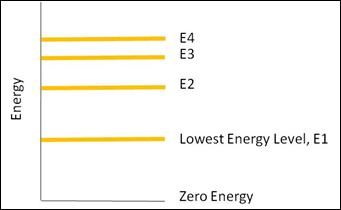
\includegraphics[width=2.2217in,height=1.3673in]{PH4CAX3V}
\end{figure}%
This Type of graph shows the energy levels that an electron \emph{can} have.
These energy levels are like a series of shelves, with each shelf
representing a different gravitational potential energy. But like a shelf
does not always have something on it, the energy level of the atom may not
have an electron at that energy. If we force an electron to go higher in
energy from a low \textquotedblleft energy shelf\textquotedblright\ by
giving it energy, it will eventually fall back down, giving up that energy
as it moves to a lower shelf. Light may provide this energy to move
electrons up to higher shelves or orbitals, and light may be given off again
when the electron falls to the lower shelf.\newline

But so far we have only dealt with individual atoms. What happens if we have
more than one atom, or a group of atoms like a solid?

Let's take two identical atoms. When they are far apart, they act as
independent systems. But when they get closer, the start acting like one
quantum mechanical system. What does that mean for the electrons in the
atoms?

From the Pauli exclusion principle, we know that they must not occupy the
same states.\begin{figure}[h!]
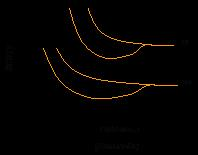
\includegraphics[width=1.9372in,height=1.5169in]{PH4CAX3W}
\end{figure}We see as the atoms get closer,
the states split. So each electron is now in a different state. Suppose we
bring 5 atoms together.\begin{figure}[h!]
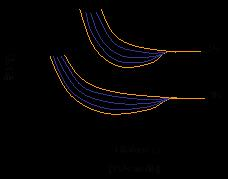
\includegraphics[width=1.9294in,height=1.5152in]{PH4CAX3X}
\end{figure}We get additional splitting of
states. Now we have five different $1s$ states. But solids have more than
five atoms. Let's bring many atoms together.\begin{figure}[h!]
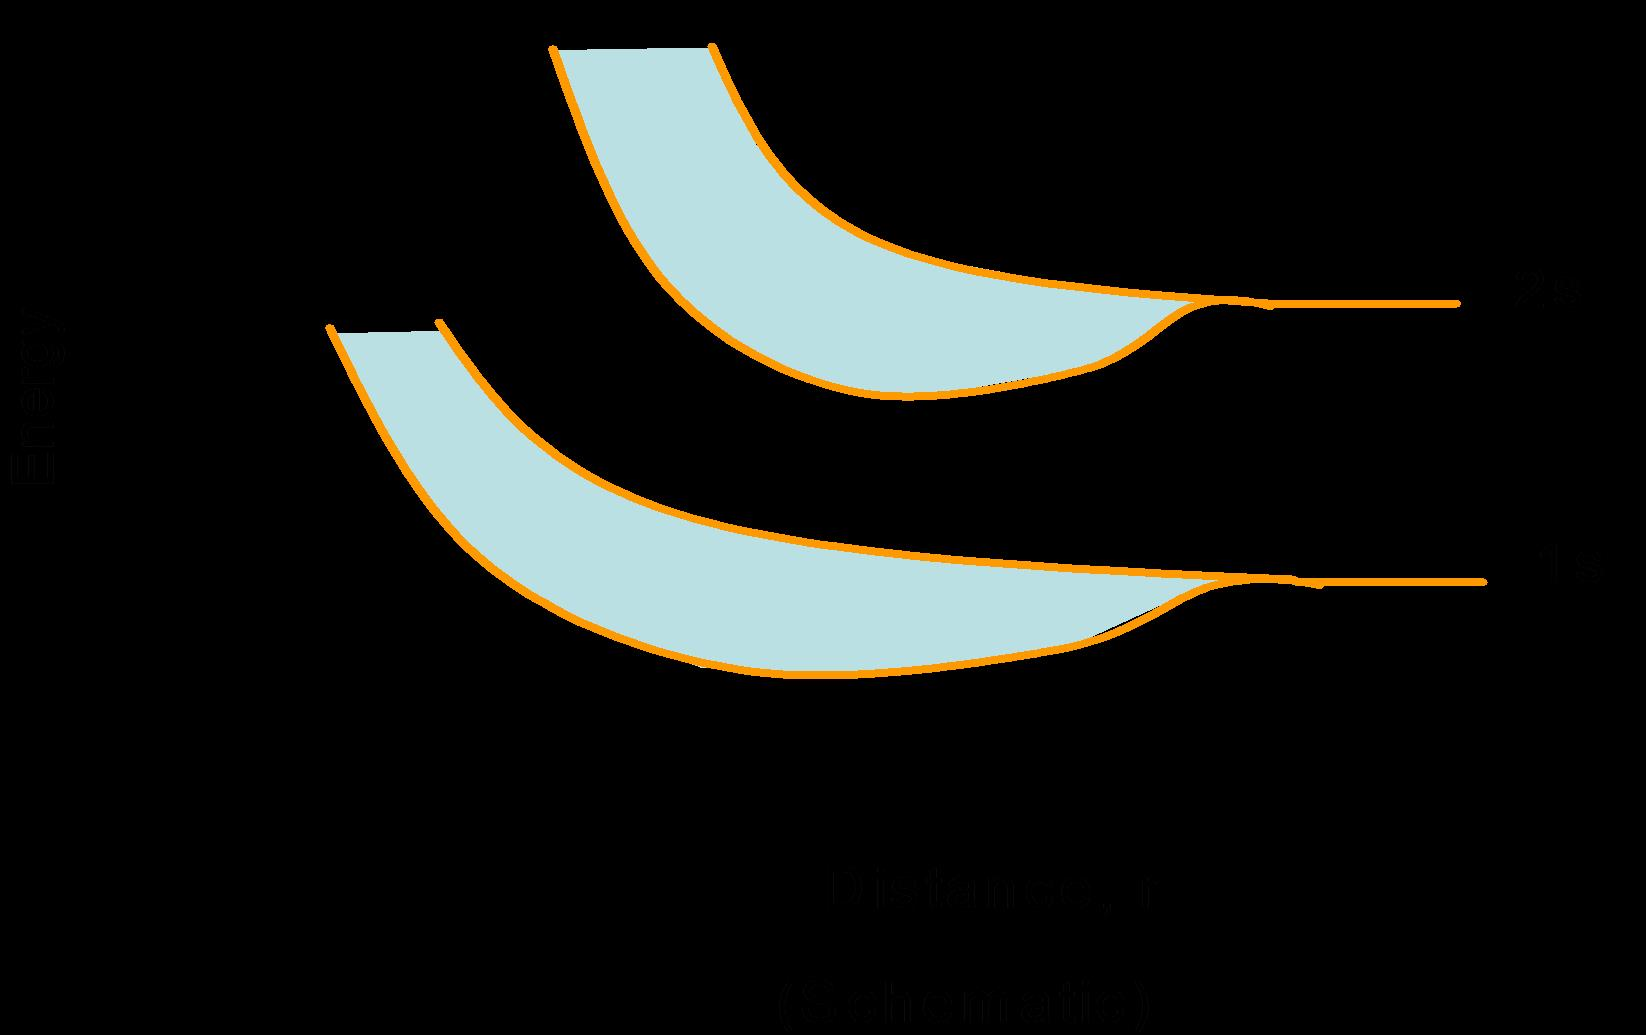
\includegraphics[width=1.8602in,height=1.4442in%
]{PH4CAX3Y}
\end{figure}Now there are so many states that
we just have a blue blur. A nearly continuous set of states in two bands.
The atoms won't allow themselves to be to close. They will reach an
equilibrium distance, $r_{o}$ where they will want to stay. \begin{figure}[h!]
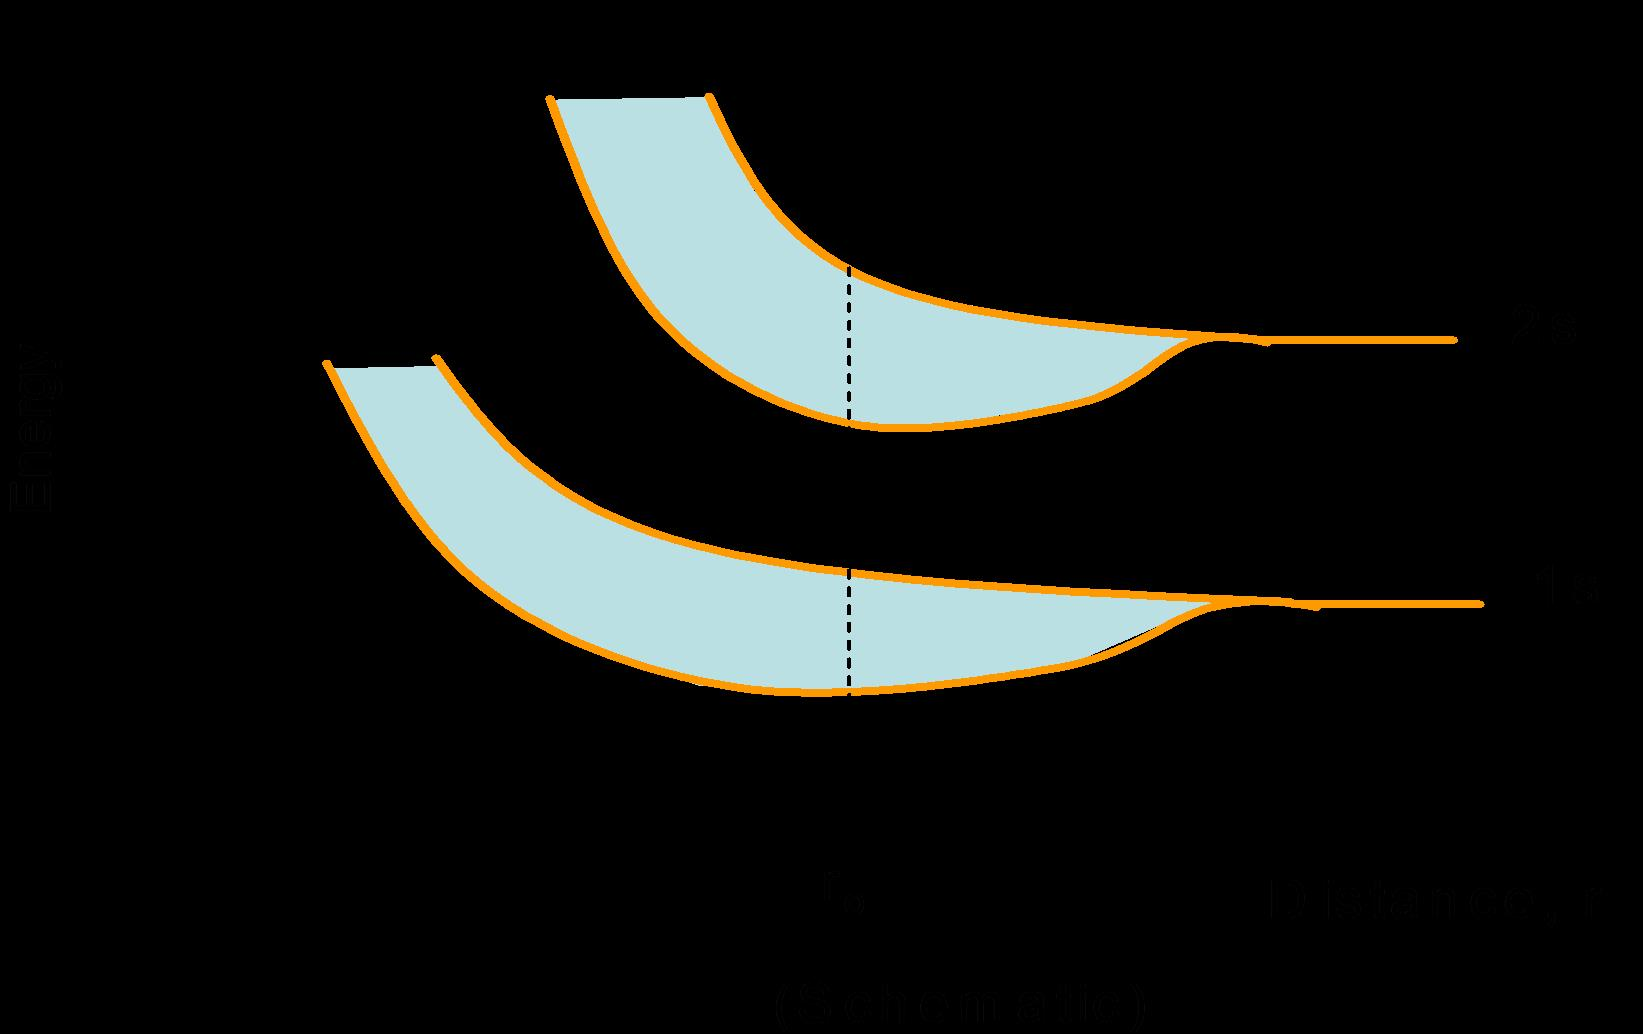
\includegraphics[width=%
1.7071in,height=1.3967in]{PH4CAX3Z}
\end{figure}%
Since this is where the atoms usually are. We will not draw the whole
diagram. We will instead just draw bands at $r_{o}.$ Here is an example.

\bigskip \begin{figure}[h!]
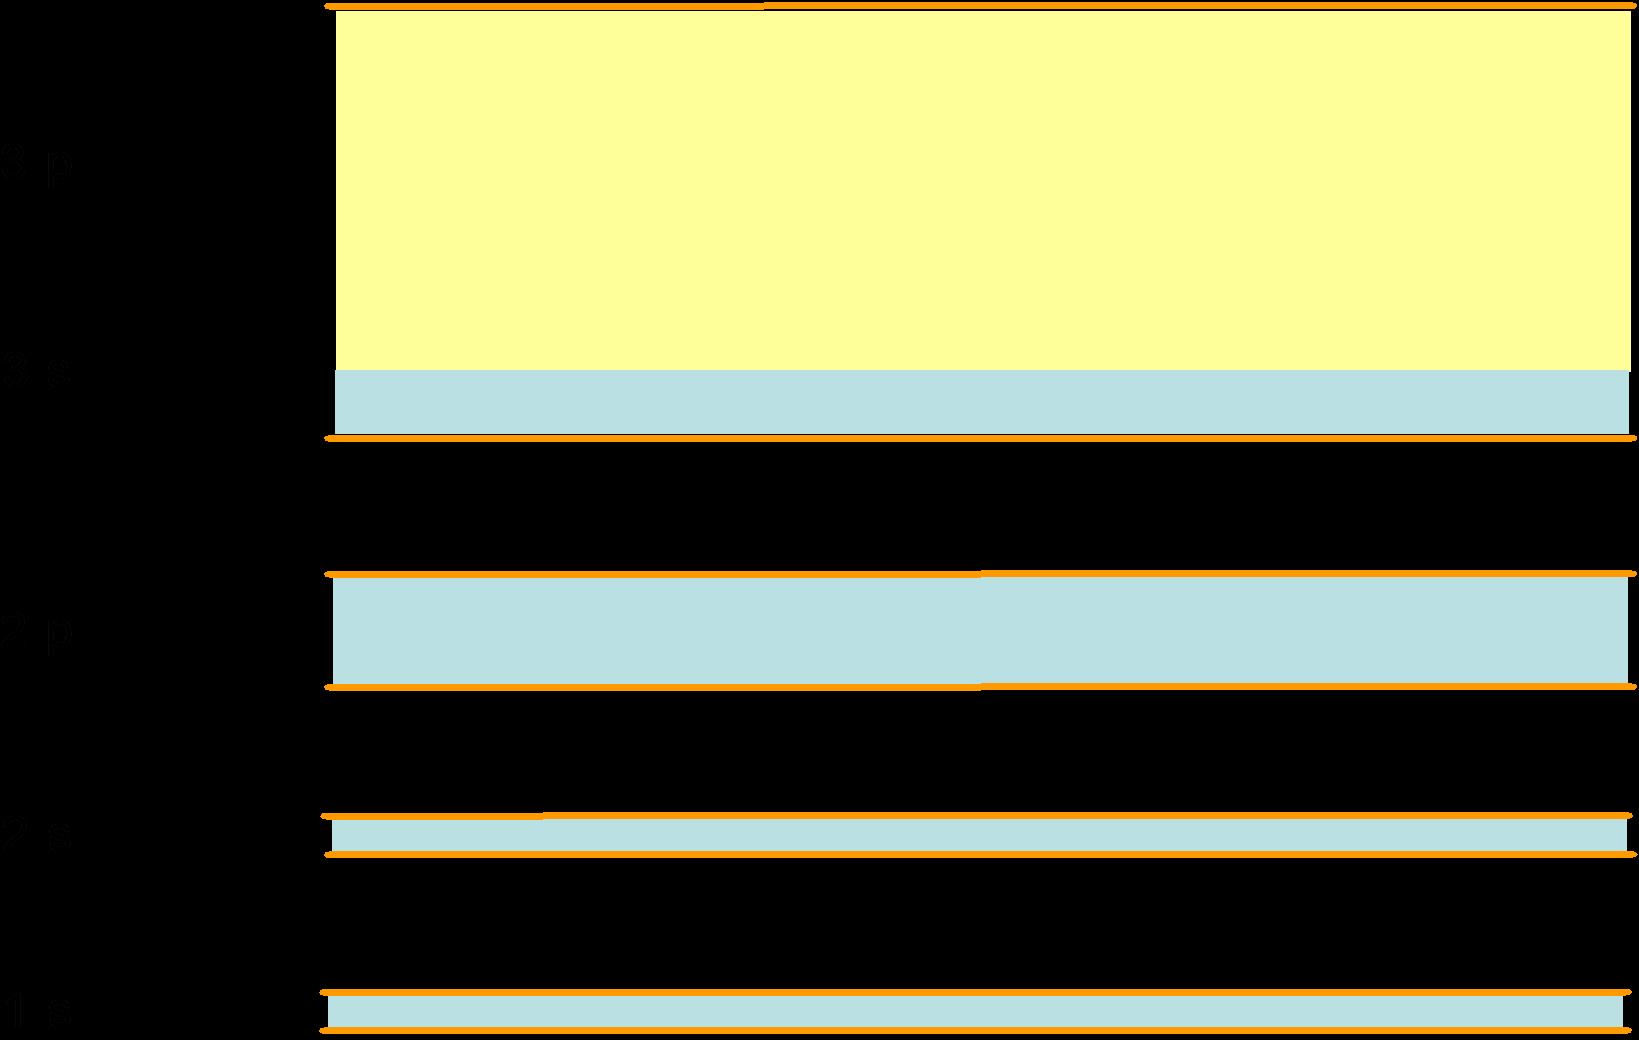
\includegraphics[width=1.9951in,height=2.1223in]{PH4CAX40}
\end{figure}

Notice that this means we have \emph{bands} of energies that are allowed,
that electrons can use, and \emph{gaps} of energy where no electron can
exist.

\section{Conduction in solids}

Notice that in our last picture, the $3s$ and $3p$ bands have grown so much
that they overlap. The situation with solids is complicated. Also notice
that the lower states are blue. We will let blue mean that they are filled.
The upper states are only partially filled. Yellow will mean empty. If we
look just at the upper bands. We will call the highest completely filled
band the \emph{valance band} and the next higher empty band the $\emph{%
conduction}$ band. We will not try to calculate the details.

We have three different conditions possible.

\subsection{Metals}

In a metal, the highest occupied band is only partially filled

\begin{figure}[h!]
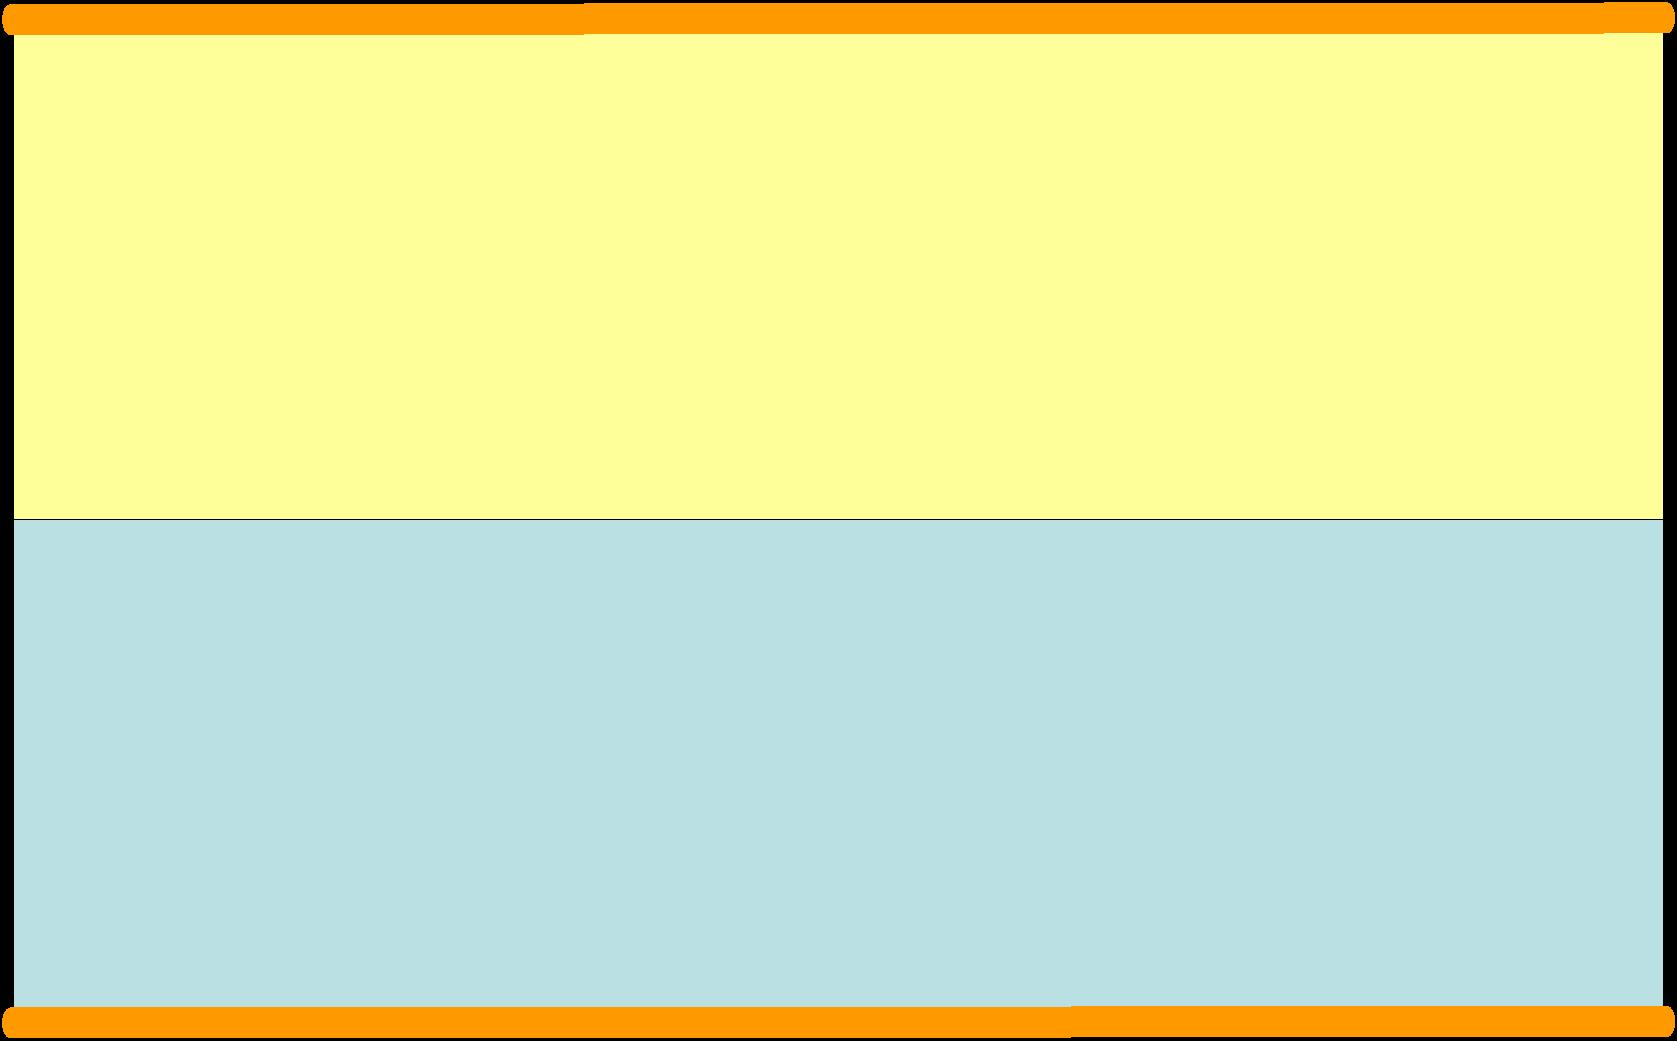
\includegraphics[width=2.0972in,height=0.6521in]{PH4CAX41}
\end{figure}

The electrons in this band require only very little energy to jump to the
next states up since they are in the same band and they are very closely
spaced. Remember that movement requires energy. So if we put a potential
difference across our metal, the electrons must be allowed to gain the extra
energy. But in the case of a metal, there are easily accessible energy
states to move to, and the electrons flow through the metal.

\subsection{Insulators}

A second condition is to have a full valance band and an empty conduction
band. The bands are separated by an energy gap of energy $E_{g}.$

\begin{figure}[h!]
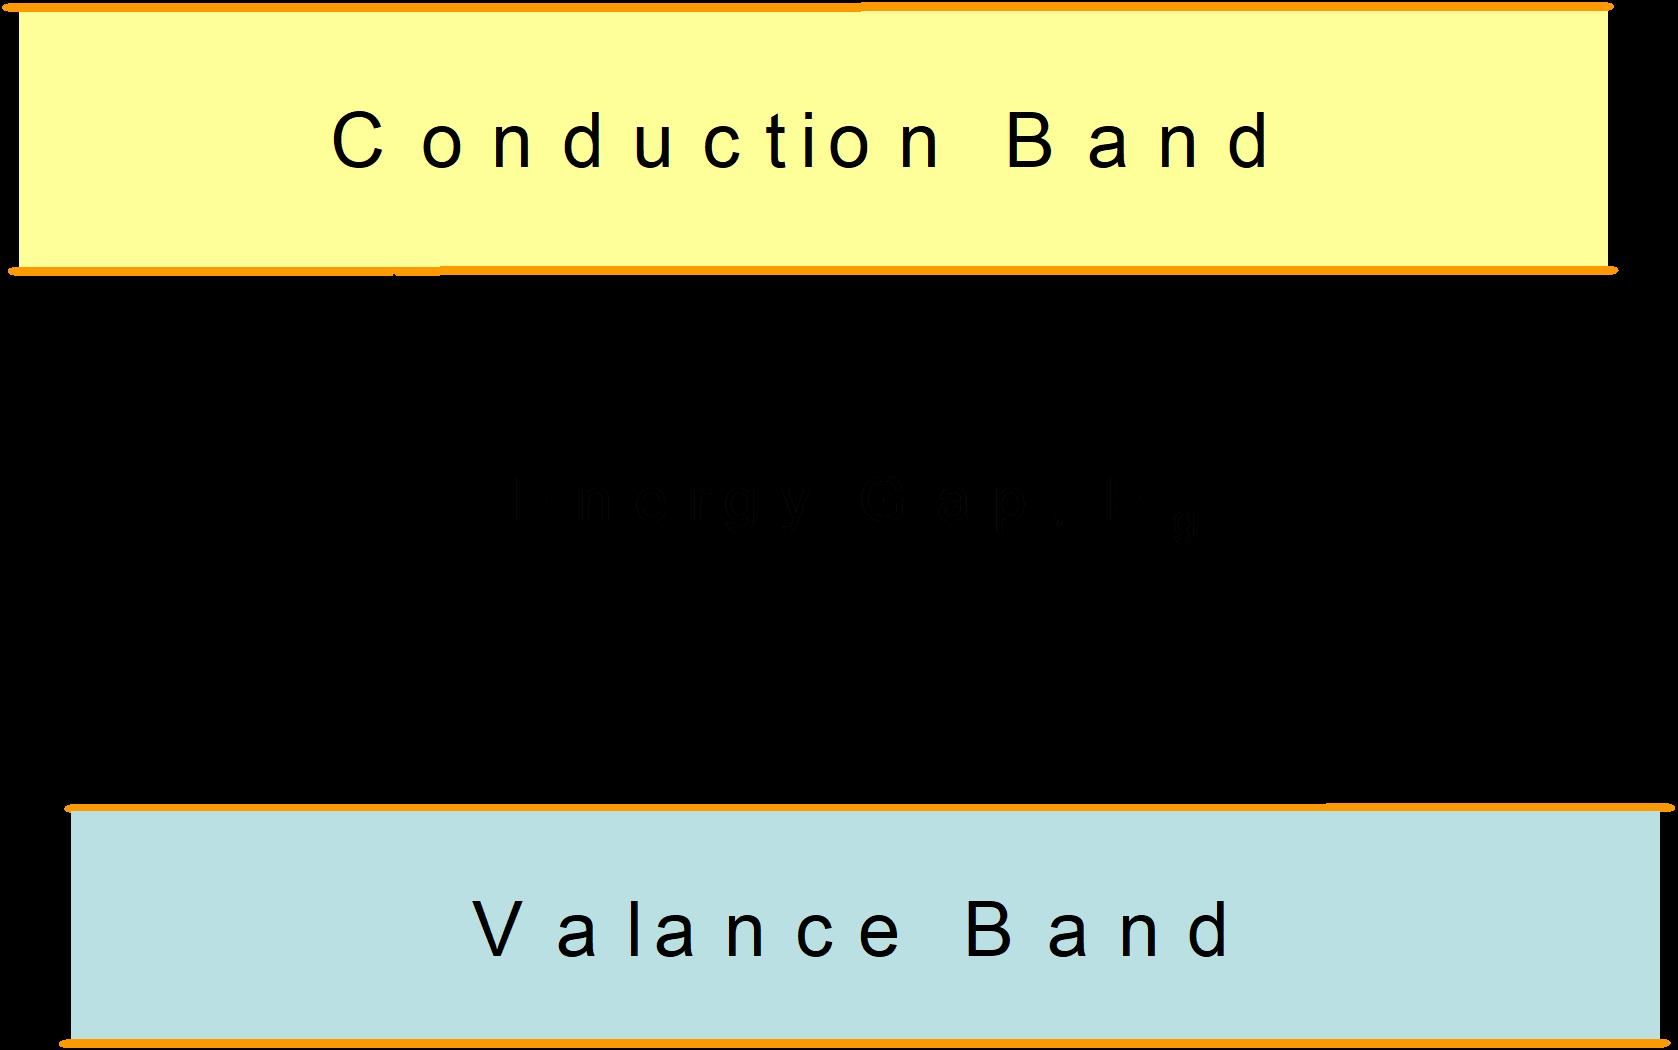
\includegraphics[width=1.6535in,height=1.7244in]{PH4CAX42}
\end{figure}In this case, a potential cannot
move the electrons, because there is no easy close energy state to move to.
If a potential is very large, then electrons can jump the gap, which is why
we said that any material can conduct, but many will not want to.

\subsection{Semiconductors}

The third condition is one where there is a band gap, but it is small. 
\begin{figure}[h!]
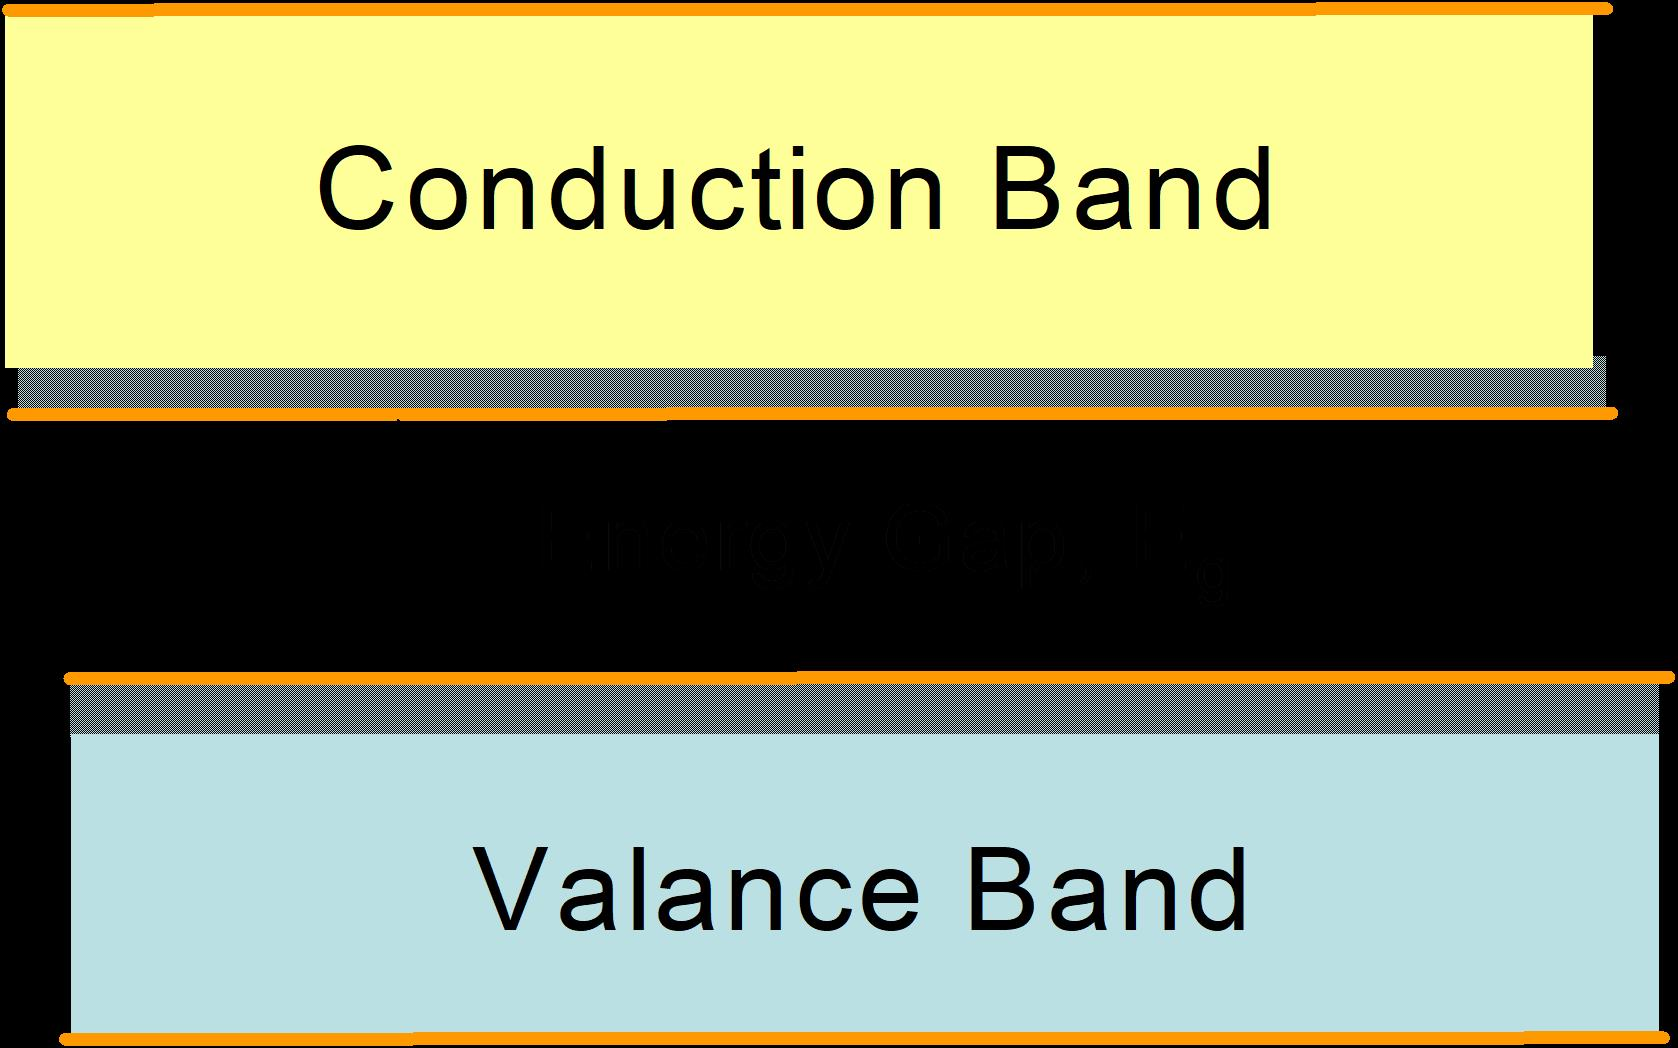
\includegraphics[width=1.6051in,height=1.0957in]{PH4CAX43}
\end{figure}If you have studied
thermodynamics you will be aware that each degree of freedom should give us 
\begin{equation*}
KE=\frac{3}{2}k_{B}T
\end{equation*}%
This is quite small for electrons, something like $0.04\unit{eV}.$ So for
insulators, at normal temperatures the thermal energy won't push electrons
across the band gap. But for semiconductors, the gap is small. At normal
temperatures, some of the electrons will cross the gap to the conduction
band. This allows them to move like electrons do in a metal. \begin{figure}[h!]
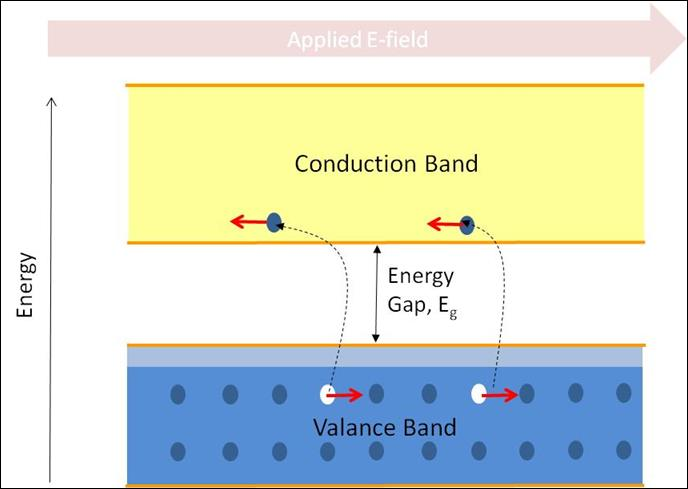
\includegraphics[width=%
2.4422in,height=1.7331in]{PH4CAX44}
\end{figure}

Notice that this leaves empty states in the valance band. Now a strange
thing happens. If we put a potential across this material, electrons from
neighboring atoms can still travel even if they are in the valance band.
They hop from one atom to the next. They fill the \textquotedblleft
holes\textquotedblright\ left by the electrons that moved to the conduction
band. Now we could say that we have two current mechanisms. One is electrons
moving in the conduction band. The other \textquotedblleft
holes\textquotedblright\ moving the other way in the valance band. Note that
\textquotedblleft holes\textquotedblright\ would be positive charge carriers.

Actually, if we add the right trace chemicals, we can control whether a
semiconductor will predominately have negative charge carriers or positive
charge carriers. If the material has predominately negative charge carriers
it is called a $n$-type semiconductor. if it has predominately positive
\textquotedblleft holes\textquotedblright\ as the charge carriers, then it
is called a $p$-type semiconductor.

\subsection{$p$-$n$ Junctions}

Let's see what happens when we put these two types of semiconductors
together. \begin{figure}[h!]
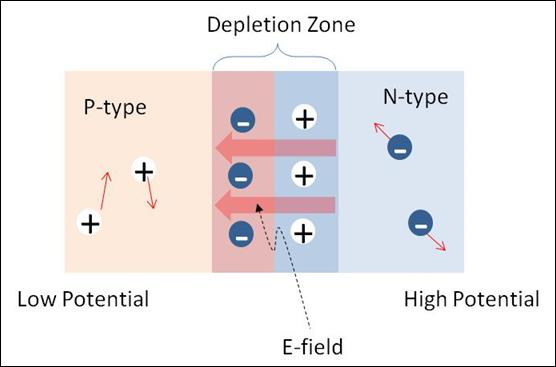
\includegraphics[width=2.5218in,height=1.663in]{PH4CAX45}
\end{figure}

You might guess that the negative and positive charge carriers would try to
combine. Electrons from the $n$ side move to the $p$ side leaving behind
positive ions. these ions can't move, they are part of the semiconductor
material. So they must stay put. Some \textquotedblleft
holes\textquotedblright\ from the $p$ side also can move. They go from the $%
p $ side to the $n$ side, leaving behind negative ions. So now in the region
marked as the \emph{depletion zone} in the figure, we have a region that has
positive charges on one side and negative charges on the other. This will
create a field in the middle with a potential difference.

You might ask why the rest of the electrons and holes don't join in. That is
because the potential that has been created stops the rest from traveling
across the border.

\subsection{Diodes}

Suppose we hook a battery to the $p$-$n$ junction so that the positive side
is connected to the $p$ side of our semiconductor junction and the $n$ side
of the semiconductor junction is connected to the negative side of the
battery. Then we would decrease the potential across the semiconductor, and
charge could then flow across the boundary.

Suppose we hook it up the other way. Then we would increase the potential,
and no charge would flow across the boundary at all.

This device is called a diode. It acts like a one-way valve for electrons.

When we hook the battery plus side to the diode $p$ side, then we say we
have given the diode a \emph{forward bias.} The other way is called \emph{%
reverse bias}.

The current equation looks a little bit familiar.%
\begin{equation*}
I=I_{o}\left( e^{\frac{q\Delta V}{k_{B}T}}-1\right)
\end{equation*}%
$\allowbreak $

and a plot looks like\begin{figure}[h!]
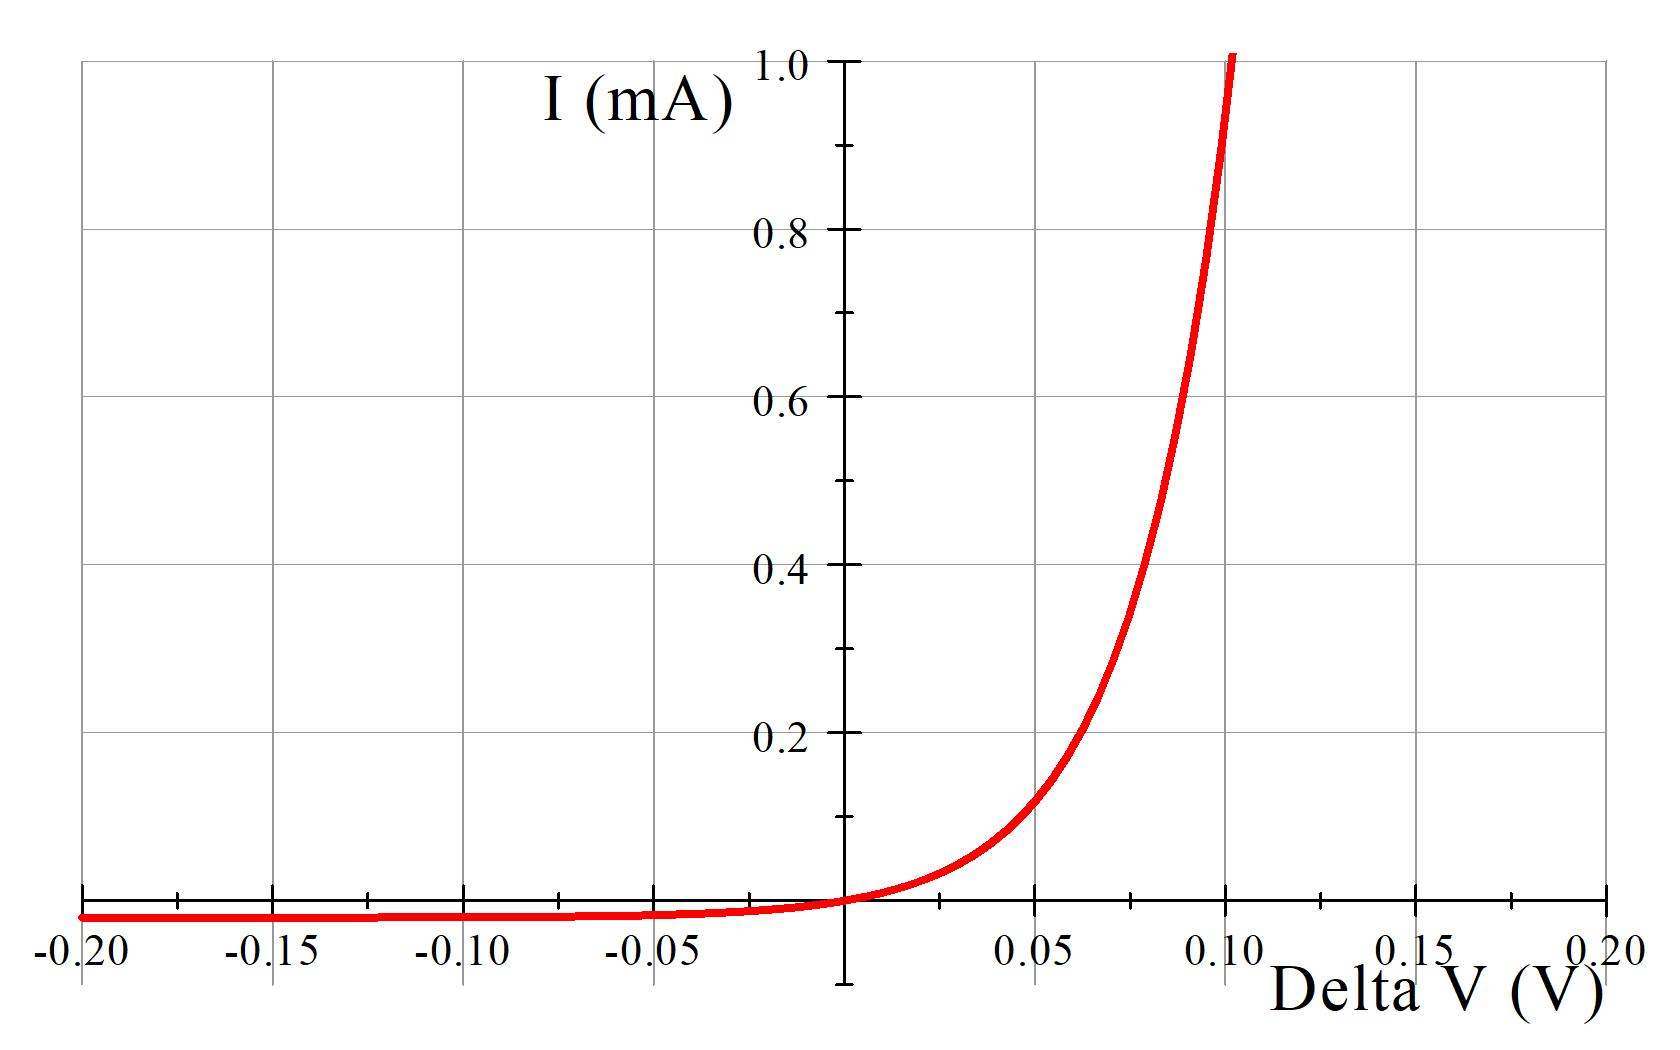
\includegraphics[width=4.0032in,height=2.6697in]{PH4CAX46}
\end{figure}

%TCIMACRO{\TeXButton{\vspace*{\fill}}{\vspace*{\fill}}}%
%BeginExpansion
\vspace*{\fill}%
%EndExpansion
\pagebreak

\section{Lab Assignment}

For this lab, you will need many hands. Work in groups of at least three,
but no more than six.

\begin{enumerate}
\item Use a light emitting diode as a transducer to form a light meter using
your voltmeter.

\item Test the following model. Light from a \textbf{point source} becomes
less intense following the formula%
\begin{equation*}
I=\frac{P}{4\pi r^{2}}
\end{equation*}%
(just like sound for you PH123 students!) so our light detector should
follow a $1/r^{2}$ like curve. You might test your light transducer by
plotting voltage (which is proportional to light intensity--do you have to
convert to intensity to show the model works) as a function of distance.

\item Work with your group to begin your proposal.

\begin{enumerate}
\item Talk to your instructor about your project, you will need instructor
approval before you start writing your proposal

\item Plan how to divide the work and, start writing a proposal for your
group project. This is a group effort. Science is done with collaboration.
So plan how you will work together and work your plan.
\end{enumerate}
\end{enumerate}

%TCIMACRO{\TeXButton{vfill}{\vfill}}%
%BeginExpansion
\vfill%
%EndExpansion